%!TEX root = ../authorinstr.tex

\section{CACLA}
A well established algorithm in Reinforcement Learning is Continuous Actor Critic Learning Automaton (CACLA)~\cite{van2007reinforcement}. The algorithm is capable of dealing with continuous state and action spaces. It implements an Actor Critic system in which both the Actor and Critic are operationalized using a Multi-Layer Perceptron. In the algorithm, the Actor is responsible for selecting the current action given the policy. The Critic is used in the calculation of the TD-error which drives the learning of the Actor. This method allows for a seperation between the representation of the policy and the value function. A visualization of the Actor-Critic system is shown in Figure~\ref{fig:actorcriticsystem}

\begin{figure}[t]
 \centering 
    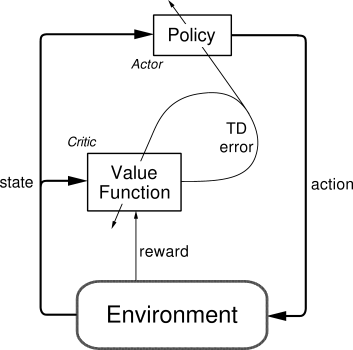
\includegraphics{figs/actorcritic.png}
 \caption{Actor Critic system. Reprinted from~\cite{sutton1998reinforcement}}
\label{fig:actorcriticsystem}
\end{figure}



